% --- PACKAGES ---
\usepackage[lyric]{songs}
\usepackage[utf8]{inputenc}
\usepackage[T1]{fontenc}
\usepackage{cochineal}
\usepackage[top=2.3cm,bottom=2.3cm,left=2.3cm,right=2.3cm]{geometry}
\usepackage[dvipsnames,table,xcdraw]{xcolor}
\usepackage{eso-pic}
\usepackage{graphicx}
\usepackage{tikz}
\usetikzlibrary{calc}
\usepackage[object=vectorian]{pgfornament}
\usepackage{fancyhdr}

%\newcommand{\SongOrnament}{%
%	\par\nointerlineskip
%	\vspace{3pt}%
%	{\centering\pgfornament[width=0.4\linewidth,color=black!60!white]{89}\par}%
%	\vspace{3pt}%
%}

% --- SONG STYLING ---
\songcolumns{2}
\columnsep=2cm
\songpos{1}
\setlength{\afterpreludeskip}{3pt}
\setlength{\versesep}{15pt plus 1pt minus 1pt}
\renewcommand\printchord[1]{{\large\sffamily\itshape\color{black!60!white}#1}}
\renewcommand{\lyricfont}{\normalfont\large}
\renewcommand{\notebgcolor}{black!13!white}
\renewcommand{\snumbgcolor}{black!20!white}
\newindex{titleidx}{titleidx}	% Adăugăm cuprins
\indexsongsas{titleidx}{\thesongnum}	% Afișează numărul cântării
\setlength{\sbarheight}{0pt}	% Delete the bar between songs

% --- COVER IMAGE COMMAND ---
\newcommand\BackgroundPic{%
	\put(0,0){%
		\parbox[b][\paperheight]{\paperwidth}{%
			\vfill
			\centering
			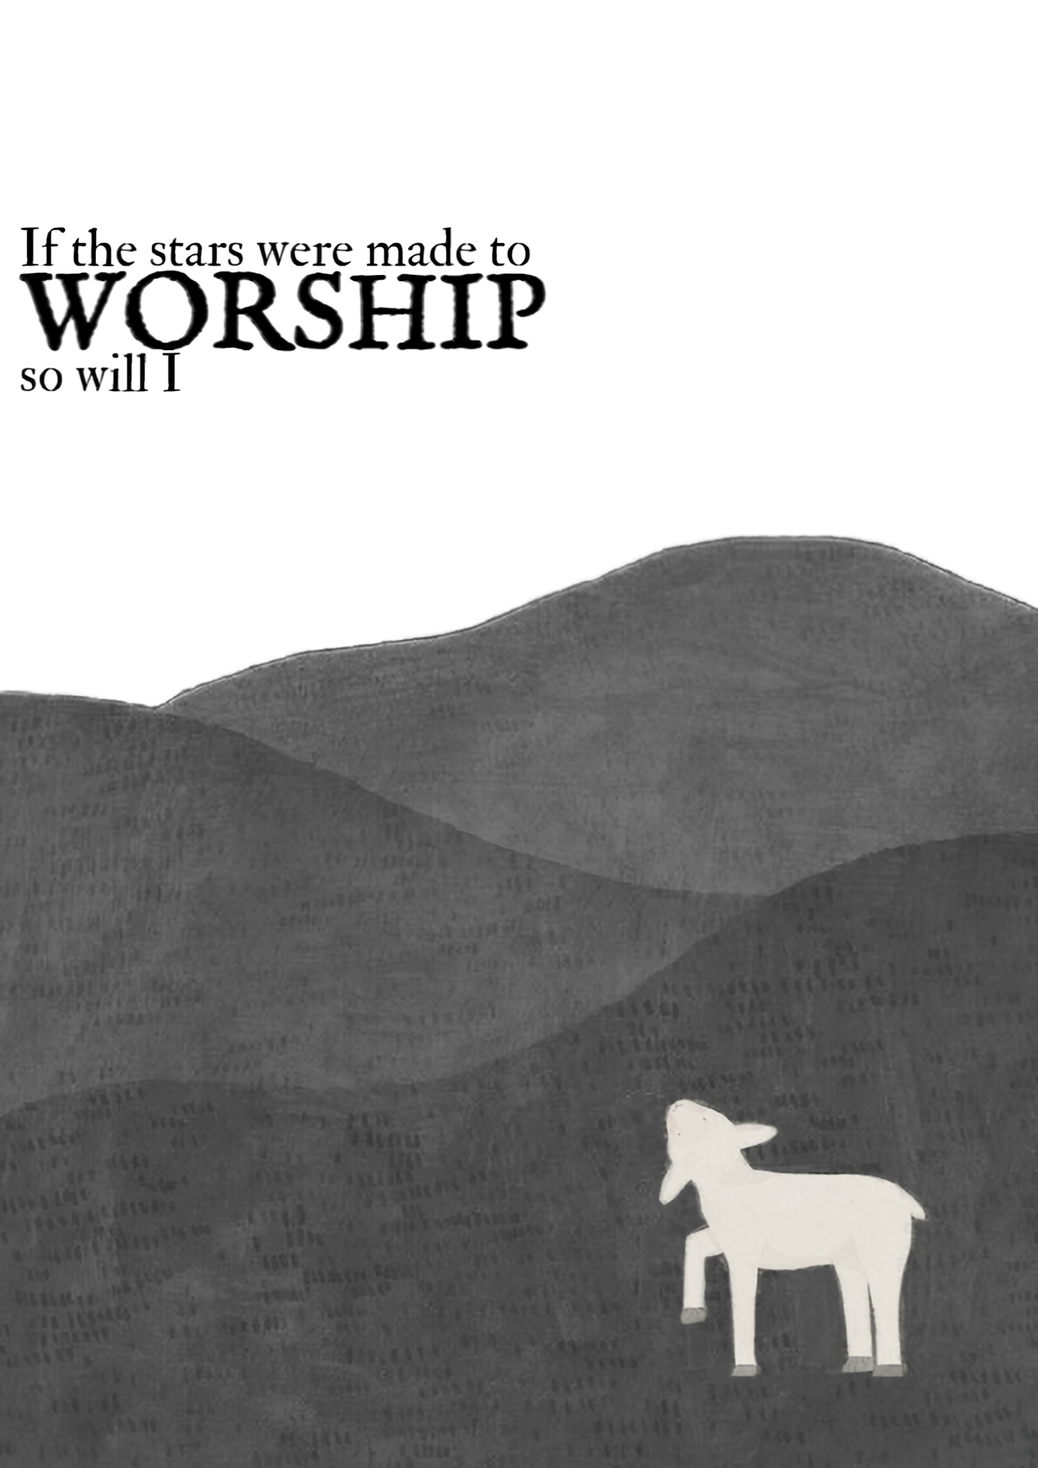
\includegraphics[width=\paperwidth]{Imagini/Copertax1_6}%
			\vfill
		}%
	}%
}

% Configure the page number footer
\pagestyle{fancy}
\fancyhf{} % Clear default headers/footers
\renewcommand{\headrulewidth}{0pt} % Remove top header line
\renewcommand{\footrulewidth}{0pt} % Remove bottom footer line

% Place the page number at the bottom center in black
\fancyfoot[C]{\small\color{black}\thepage}
\setlength{\footskip}{12pt} % Adjusts distance between lyrics and page number

% --- PAGE BORDER COMMAND (Ornament 61 + 87/89 in Chord Color) ---
\newcommand{\PageBorder}{%
	\begin{tikzpicture}[
		remember picture, 
		overlay, 
		every node/.style={inner sep=0pt}
		]
		% Se poate folosi 1 cm la shift
		% #1 pgornament pt colțuri: 61
		% #2 pgornament pt colturi: 37
		% #3 pgornament pt colturi: 41
		% #4 pgornament pt colturi: 63
		% Colțul Stânga-Sus
		\node[shift={(0.5cm,-0.5cm)},anchor=north west](CNW)	
		at (current page.north west) {\pgfornament[width=1.5cm,color=black!60!white]{41}};
		
		% Colțul Dreapta-Sus (oglindit pe verticală)
		\node[shift={(-0.5cm,-0.5cm)},anchor=north east](CNE)
		at (current page.north east) {\pgfornament[width=1.5cm,symmetry=v,color=black!60!white]{41}};
		
		% Colțul Stânga-Jos (oglindit pe orizontală)
		\node[shift={(0.5cm,0.5cm)},anchor=south west](CSW)
		at (current page.south west) {\pgfornament[width=1.5cm,symmetry=h,color=black!60!white]{41}};
		
		% Colțul Dreapta-Jos (oglindit pe ambele axe: v și h)
		\node[shift={(-0.5cm,0.5cm)},anchor=south east](CSE)
		at (current page.south east) {\pgfornament[width=1.5cm,symmetry=v,symmetry=h,color=black!60!white]{41}};
		
		% Varianta 1
		% Liniile orizontale (Sus și Jos)
		%\pgfornamentline[color=black!60!white]{CNW.north east}{CNE.north west}{3}{87}
		%\pgfornamentline[color=black!60!white]{CSW.south east}{CSE.south west}{3}{87}
		
		% Liniile verticale (Stânga și Dreapta - corectat punctul final din dreapta jos!)
		%\pgfornamentline[color=black!60!white]{CNW.south west}{CSW.north west}{4}{87}
		%\pgfornamentline[color=black!60!white]{CNE.south east}{CSE.north east}{4}{87}
		
		% Varianta 2
		% Liniile orizontale (Sus și Jos)
		\pgfornamentline[color=black!60!white]{CNW.north east}{CNE.north west}{3}{88}
		\pgfornamentline[color=black!60!white]{CSW.south east}{CSE.south west}{3}{88}
		
		% Liniile verticale (Stânga și Dreapta - corectat punctul final din dreapta jos!)
		\pgfornamentline[color=black!60!white]{CNW.south west}{CSW.north west}{4}{88}
		\pgfornamentline[color=black!60!white]{CNE.south east}{CSE.north east}{4}{88}
	\end{tikzpicture}%
}